\begin{appendix}
%\chapter{Les micromodules}
%\label{a_micro}
\chapter{Compression MDL}
\label{an:compression}

\section{Fonction de distance}
\label{an:compression_dist}

Pour réaliser du clustering sur des segments de trajectoires, Jae-Gil Lee et Kyu-Young Whang ont défini une notion de distance composée de trois composantes comme suit : la distance perpendiculaire ($d_{\perp}$), la distance parallèle ($d_{\parallel}$) et la distance angulaire ($d_{\theta}$). Elles sont illustrées de manière intuitive dans la Figure~\ref{fig:distancesA}. Elles sont définies formellement de la façon suivante. 

Supposons que nous ayons 2 segments en $n$ dimensions, $L_i = s_i e_i$ et $L_j = s_j e_j$, où $s_i$, $e_i$, $s_j$ et $e_j$ représentent des points de $n$ dimensions. Nous assignons le segment plus long à $L_i$ et le segment plus court à $L_j$.


\begin{figure}[ht]
    \centering
    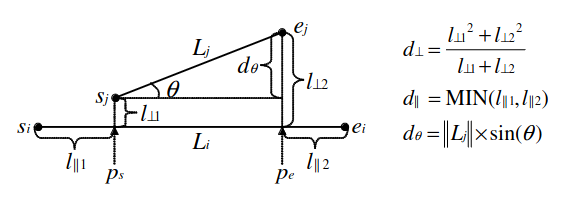
\includegraphics[width=0.44\textwidth]{Images/distances.png}
    \caption{Les 3 composantes de distance entre 2 segments}
    \label{fig:distancesA}
    Source : \href{https://hanj.cs.illinois.edu/pdf/sigmod07_jglee.pdf}{Trajectory Clustering: A Partition-and-Group Framework}
\end{figure}

\begin{enumerate}
    \item La distance perpendiculaire $d_{\perp}$ :
        \begin{equation}
            d_{\perp}(L_i, L_j) = \frac{l_{\perp 1}^2 + l_{\perp 2}^2}{l_{\perp 1} + l_{\perp 2}},
        \end{equation}
        où $l_{\perp 1}$ est la distance euclidienne entre $\overrightarrow{sj}$ et le point de projection $p_s$ de $\overrightarrow{sj}$ sur $L_i$, et $l_{\perp 2}$ est la distance euclidienne entre $\overrightarrow{ej}$ et le point de projection $p_e$ de $\overrightarrow{ej}$ sur $L_i$.



    \item La distance parallèle $d_{\parallel}$ est définie comme :
        \begin{equation}
            d_{\parallel}(L_i, L_j) = \min(l_{\parallel 1}, l_{\parallel 2}),
        \end{equation}
        où $l_{\parallel 1}$ est la distance euclidienne minimale entre $p_s$ et $\overrightarrow{si}$ ou $\overrightarrow{ei}$, et $l_{\parallel 2}$ est la distance euclidienne minimale entre $p_e$ et $\overrightarrow{si}$ ou $\overrightarrow{ei}$.


    \item La distance d'angle $d_{\theta}$ est définie comme :
        \begin{equation}
            d_{\theta}(Li, Lj ) =
            \begin{cases}
                \| Lj \| \times \sin({\theta}), & \text{si } 0^\circ \le {\theta} < 90^\circ\ \\
                \| Lj \|, & si \hspace{0.3cm} 90^\circ \le {\theta} \le 180
            \end{cases}
        \end{equation}

        où $\theta$ est l'angle d'intersection le plus petit entre $L_i$ et $L_j$ et $\| L_j \|$ est la longueur de $L_j$.

        %‖ Lj ‖


\end{enumerate}

\vspace{0.5cm}
Nous définissons finalement la distance entre deux segments de droite comme suit : 

\[
\mathrm{dist}(L_i,L_j) = w_\perp \cdot d_\perp(L_i,L_j) + w_{\parallel} \cdot d_{\parallel}(L_i,L_j) + w_\theta \cdot d_\theta(L_i,L_j)
\]

Les poids $w_\perp$, $w_{\parallel}$ et $w_\theta$ seront à déterminer en fonction des applications. Dans notre cas, nous les fixerons défaut à 1, car selon l'auteur ces valeurs fonctionnent généralement bien dans de nombreuses applications et ensembles de données.

%%%%%%%%%%%%%%%%%%%%%%%%%%%%%%%%%%%%%%%%%
\section{Compression en temps linéaire}
\label{an:compression_lin}

La méthode proposée consiste à considérer que l'ensemble des optima locaux est l'optimum global. On définira $MDLpar(p_i, p_j)$ le coût MDL ($ L(H) + L(D|H) $) d'une trajectoire entre pi et pj (i<j) en supposant que pi et pj sont les seuls points caractéristiques. Et MDLnopar(pi, pj) le coût MDL en supposant que tous les points de pi à pj sont caractéristiques, autrement dit, en préservant la trajectoire originale. Notons que dans MDLnopar(pi, pj), $L(D|H)$ est nul. Un optimum local est la partition de trajectoire pipj la plus longue qui satisfait MDLpar(pi, pk) $\le$ MDLnopar(pi, pk) pour tout k tel que $i < k \le j$. Si le premier est inférieur au second, cela signifie que choisir pk comme point caractéristique rend le coût de MDL plus petit que de ne pas le choisir.

%Approximate Trajectory Partitioning
L'algorithme fonctionne de la manière suivante :

\begin{enumerate}
    \item Nous calculons MDLpar et MDLnopar pour chaque point d'une trajectoire. 
    \item Si MDLpar est supérieur à MDLnopar, nous insérons le point précédent immédiat dans l'ensemble des points caractéristiques. Et nous répétons la même procédure à partir de ce point. 
    \item Sinon, nous augmentons la longueur d'une partition de trajectoire candidate. Et on continue
\end{enumerate}

%%%%%%%%%%%%%%%%%%%%%%%%%%%%%%%%%%%%%%%%%
%%%%%%%%%%%%%%%%%%%%%%%%%%%%%%%%%%%%%%%%%
\chapter{Propagation d'affinité}
\section{Implémentation}
\label{an:propa}
\subsubsection{Comment avons-nous implémenté cet algorithme ?}
Par soucis de lisibilité, notons :


\begin{itemize}
    \item S, la matrice de similarité.
    \item R, la matrice de responsabilité.
    \item D, la matrice de disponibilité.
\end{itemize}
% \begin{multicols}{2}
    \hspace*{13px} La structure de nos matrices est faite pour pouvoir comparer un élément d'index I à un élément d'index J, il est donc nécessaire d'utiliser une structure de liste ordonnée et fixe.\\
    Pour commencer, il nous faut remplir la matrice de similarité.
    Chacun de nos objets donnés est capable au préalable de se comparer à d'autres objets du même type.\\
    Une méthode distance nous permet donc de comparer un objet I à un objet J. \\ 
    (Voir l'algorithme implémenté \ref{sec:simcalc})\\
    % \begin{algorithmic}[1]
    %     % \State $\texttt{Méthode de calcul de la similarité$
    %     \State $E \gets \texttt{L'ensemble d'éléments}$
    %     \State $T \gets \texttt{la taille de E}$
    %     \State $S \gets \texttt{Une matrice de taille T*T}$
    %     \For{\texttt{I allant de 0 à T}}
    %         \For{\texttt{J allant de 0 à T}}
    %             \State $S(I,J) \gets \texttt{E(I).distance(E(J))}$
    %         \EndFor
    %     \EndFor
    % \end{algorithmic}
% \end{multicols}

% \begin{multicols}{2}
    Mettre à jour la matrice de responsabilité se fait une fois la similarité calculée. (voir figure \ref{fig:responsibility})\\
    De manière plus explicite, la responsabilité d'un élément i par rapport à k se calcule par sa valeur de similarité, moins la valeur maximale de la disponibilité pour les éléments i en considérant tous les autres points de données j, sauf l'élément k. De cette manière, nous pouvons quantifier l'importance d'un élément pour les autres éléments.\\
    (Voir l'algorithme implémenté \ref{sec:rescalc})\\
    % \begin{algorithmic}[1]
    %     % \State $\texttt{Méthode de calcul de la responsabilité$
    %     \State $E \gets \texttt{L'ensemble d'éléments}$
    %     \State $T \gets \texttt{la taille de E}$
    %     \State $S \gets \texttt{Une matrice de taille T*T}$
    %     \For{\texttt{I allant de 0 à T}}
    %         \For{\texttt{J allant de 0 à T}}
    %             \State $V = \texttt{S[i] + D[i]}$
    %             \State $V[i] = -\infty$ 
    %             \State $V[k] = -\infty$
    %             \State $R[i,k] = R[i,k] + (S[i,k] - max(v))$
    %         \EndFor
    %     \EndFor
    % \end{algorithmic}
    
    \hspace*{13px} Un paramètre que nous avons nommé "damping" est un paramètre d'amortissement compris entre 0 et 1 qui contrôle la quantité de propagation d'affinité entre les éléments. Nous l'appliquons à la formule de cette manière :\\ 
    \begin{equation}
        \begin{aligned}
            R\left ( i,k \right ) = R\left ( i,k \right ) * damping + S\left ( i,k \right ) - (1 - damping) * max\left \{ D\left ( i,k' \right ) + S\left ( i,k' \right ) \right \}
        \end{aligned}
    \end{equation}\\
    Plus ce paramètre tend vers 0, plus les éléments similaires ne seront regroupés qu'avec leurs voisins directs. Au contraire, plus le damping est proche de 1, plus les points de données similaires seront regroupés ensemble, indépendamment de leur position dans l'ensemble des éléments.\\
    
    Mettre à jour la matrice de disponibilité se fait une fois la responsabilité mise à jour. \\ 
    (Voir l'algorithme implémenté \ref{sec:avacalc})\\
    % \begin{algorithmic}[1]
    %     \State $E \gets \texttt{L'ensemble d'éléments}$
    %     \State $T \gets \texttt{la taille de E}$
    %     \State $R \gets \texttt{Une matrice de taille T*T}$
    %     \For{\texttt{I allant de 0 à T}}
    %         \For{\texttt{J allant de 0 à T}}
    %             \State $V \gets \texttt{prendre colone k dans R}$
    %             \If{$i\neq k$} 
    %                 \State $V[i] = -\infty$ 
    %                 \State $V[k] = -\infty$
    %                 \State $V[V < 0] = 0$
    %                 \State $D[i,k] = D[i,k] + min(0, R[k,k] + somme(V))$
    %             \Else
    %                 \State $V[k] = -\infty$
    %                 \State $V[V < 0] = 0$
    %                 \State $D[k,k] = D[k,k] + somme(V)$
    %             \EndIf
    %         \EndFor
    %     \EndFor
    % \end{algorithmic}
    R(k,k) est l'élément de la matrice de responsabilité R correspondant à la similarité entre le point k et lui-même. La somme est prise sur tous les points de données i' autres que i et j, et mesure l'influence des autres points de données sur la disponibilité du point i pour être affecté au 
    cluster contenant le point j. La fonction max est utilisée ici pour ne prendre en compte que les valeurs positives de la matrice de responsabilité, ne considérant donc que les éléments i' qui ont une similarité positive avec le point k. Enfin, la fonction min est là pour contraindre le résultat final à être négatif ou nul. Cela permet de quantifier l'importance des autres éléments pour un élément donné.\\
    \hspace*{13px} Une fois le processus de mise à jour de la responsabilité et la disponibilité répété un certain nombre de fois, nous finissons par faire l'addition matricielle de la matrice de responsabilité avec celle de disponibilité pour pouvoir en extraire les clusters et leur représentant, nous appelons cette matrice la matrice de critère. La valeur de critère la plus élevée de chaque colonne est désignée comme exemplaire et les colonnes qui partagent le même exemplaire se trouvent dans le même cluster.\\
    \hspace*{13px} Le processus de mise à jour de la responsabilité et la disponibilité sont exécutés un nombre arbitrairement de fois dans notre implémentation. Cependant, cet algorithme converge relativement rapidement, calculer la matrice de critère à chaque itération permettrait de détecter une convergence et ainsi éviter de réaliser des itérations inutiles. \\

\section{Méthode de calcul de la similarité}
\label{sec:simcalc}
\begin{algorithmic}[1]
    % \State $\texttt{Méthode de calcul de la similarité$
    \State $E \gets \texttt{L'ensemble d'éléments}$
    \State $T \gets \texttt{la taille de E}$
    \State $S \gets \texttt{Une matrice de taille T*T}$
    \For{\texttt{I allant de 0 à T}}
        \For{\texttt{J allant de 0 à T}}
            \State $S(I,J) \gets \texttt{E(I).distance(E(J))}$
        \EndFor
    \EndFor
\end{algorithmic}

\section{Méthode de calcul de la responsabilité}
\label{sec:rescalc}
\begin{algorithmic}[1]
    % \State $\texttt{Méthode de calcul de la responsabilité$
    \State $E \gets \texttt{L'ensemble d'éléments}$
    \State $T \gets \texttt{la taille de E}$
    \State $S \gets \texttt{Une matrice de taille T*T}$
    \For{\texttt{I allant de 0 à T}}
        \For{\texttt{J allant de 0 à T}}
            \State $V = \texttt{S[i] + D[i]}$
            \State $V[i] = -\infty$ 
            \State $V[k] = -\infty$
            \State $R[i,k] = R[i,k] + (S[i,k] - max(v))$
        \EndFor
    \EndFor
\end{algorithmic}

\newpage
\section{Méthode de calcul de la disponibilité}
\label{sec:avacalc}
\begin{algorithmic}[1]
    \State $E \gets \texttt{L'ensemble d'éléments}$
    \State $T \gets \texttt{la taille de E}$
    \State $R \gets \texttt{Une matrice de taille T*T}$
    \For{\texttt{I allant de 0 à T}}
        \For{\texttt{J allant de 0 à T}}
            \State $V \gets \texttt{prendre colone k dans R}$
            \If{$i\neq k$} 
                \State $V[i] = -\infty$ 
                \State $V[k] = -\infty$
                \State $V[V < 0] = 0$
                \State $D[i,k] = D[i,k] + min(0, R[k,k] + somme(V))$
            \Else
                \State $V[k] = -\infty$
                \State $V[V < 0] = 0$
                \State $D[k,k] = D[k,k] + somme(V)$
            \EndIf
        \EndFor
    \EndFor
\end{algorithmic}





\end{appendix}